\chapter{考察}\label{cha:Discussion}
本研究では、電子フォーム作成時間の削減を目的としたラベル付き記入欄検出手法の提案を行った。
本提案手法は、以下に示す2つの機能を持つ。

\begin{itemize}
  \item ラベル付き領域座標取得機能
  \item 領域描画画像出力機能
\end{itemize}

5章では、本提案手法が持つ2つの機能について、正しく動作することを確認した。
本章では、まず、本提案手法の有用性について考察する。次に、本提案手法と関連研究を比較する。最後に、本提案手法の問題点について述べる。

\section{本提案手法の有用性に関する評価}\label{sec:evalue_usefulness}
本提案手法の有用性を評価するため、本提案手法を、電子フォーム作成ツールであるPhotolizeに適用し、実験を行う。
Photolizeは、スマートフォンで撮影した帳票の画像に対して、電子フォーム記入欄を配置することによって、電子フォームを作成するサービスである\cite{Photolize}。
本提案手法をPhotolizeに適用することで、帳票画像記入欄を検出し、領域座標とラベルをまとめたJSONファイルから、電子フォーム記入欄を配置する手間と時間を削減することができる。

実験は、2枚の帳票画像に対して本提案手法を適用し、検出できなかった帳票画像記入欄や、誤検出によって電子フォーム記入欄に対して、被験者には、Photolizeを利用し、電子フォーム記入欄を配置してもらう。
実験の対象とした帳票の画像を、図\ref{fig:experiment_A}と図\ref{fig:experiment_B}に示す。
図\ref{fig:experiment_A}は、本提案手法が入力の対象とする帳票画像のうち、電子文書の画像であり、図\ref{fig:experiment_B}は、電子化文書の画像である。
以降、図\ref{fig:experiment_A}の画像を、帳票画像A、図\ref{fig:experiment_B}の画像を、帳票画像Bと呼ぶ。

\begin{figure}[t]
    \begin{center}
        \fbox{
            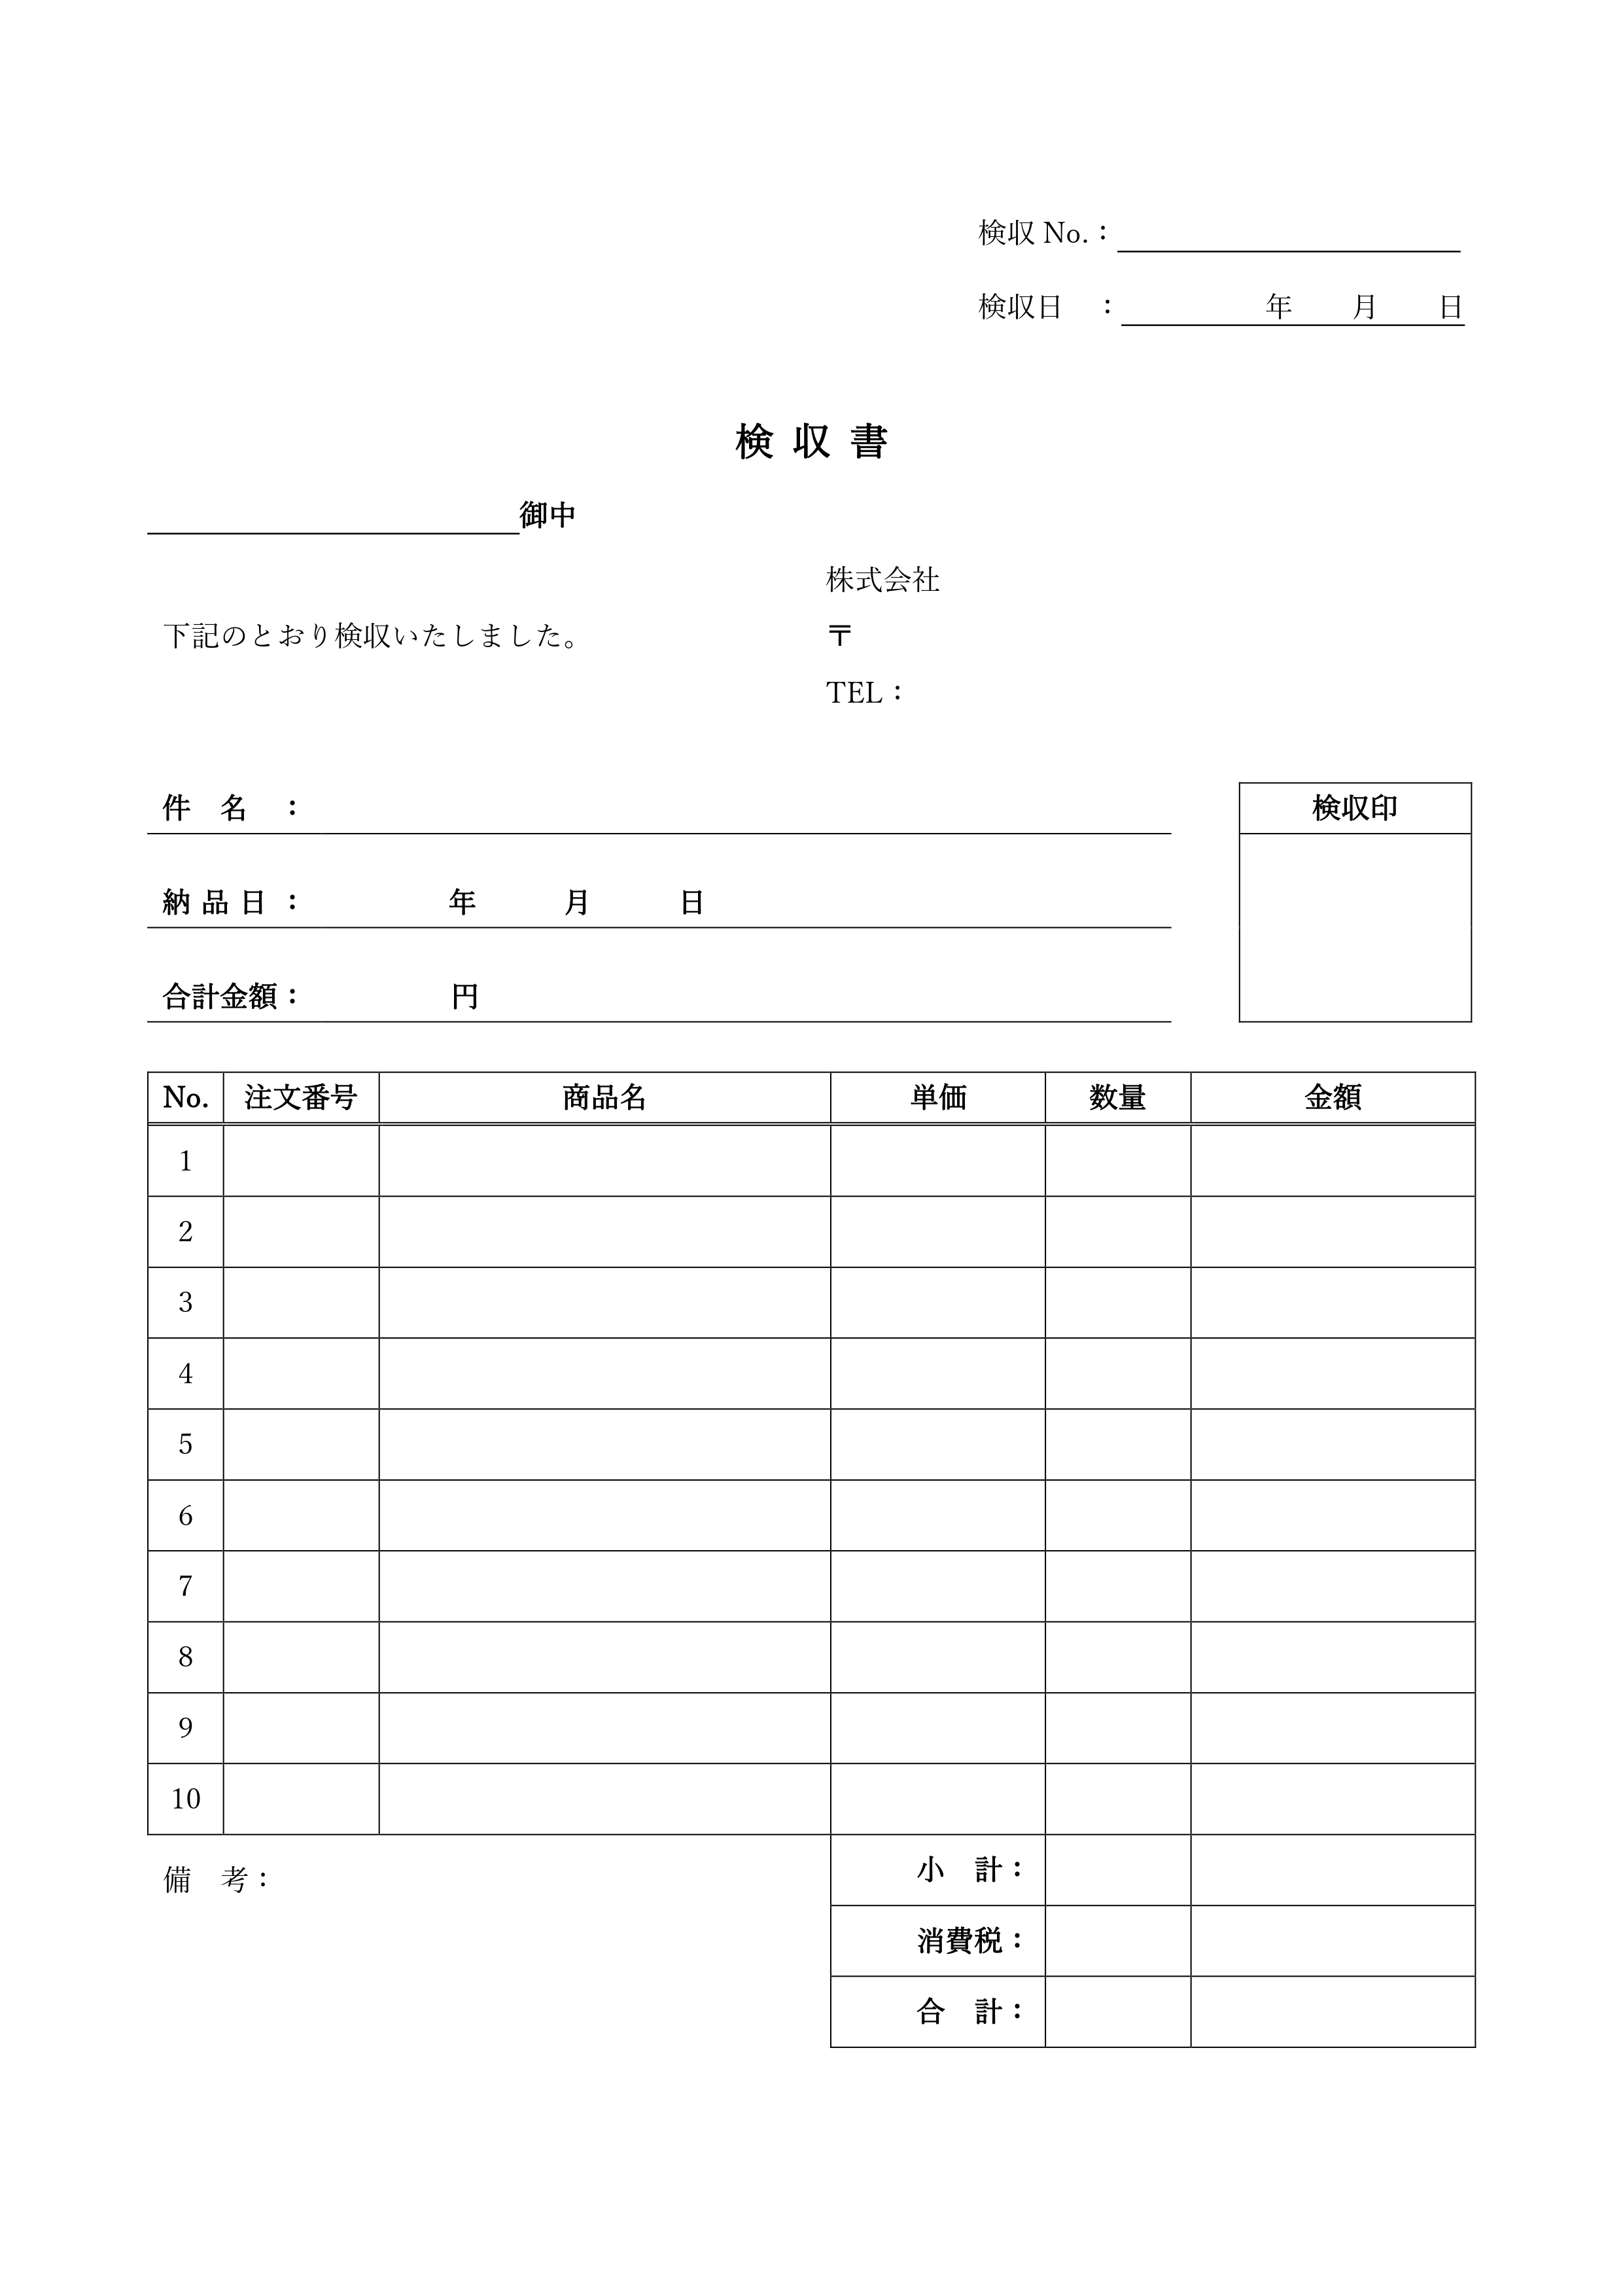
\includegraphics[width=15cm]{image/06-discussion/experiment_A.jpg}
            }
        \caption{実験対象である帳票画像A}
        \label{fig:experiment_A}
    \end{center}
\end{figure}

\begin{figure}[t]
    \begin{center}
        \fbox{
            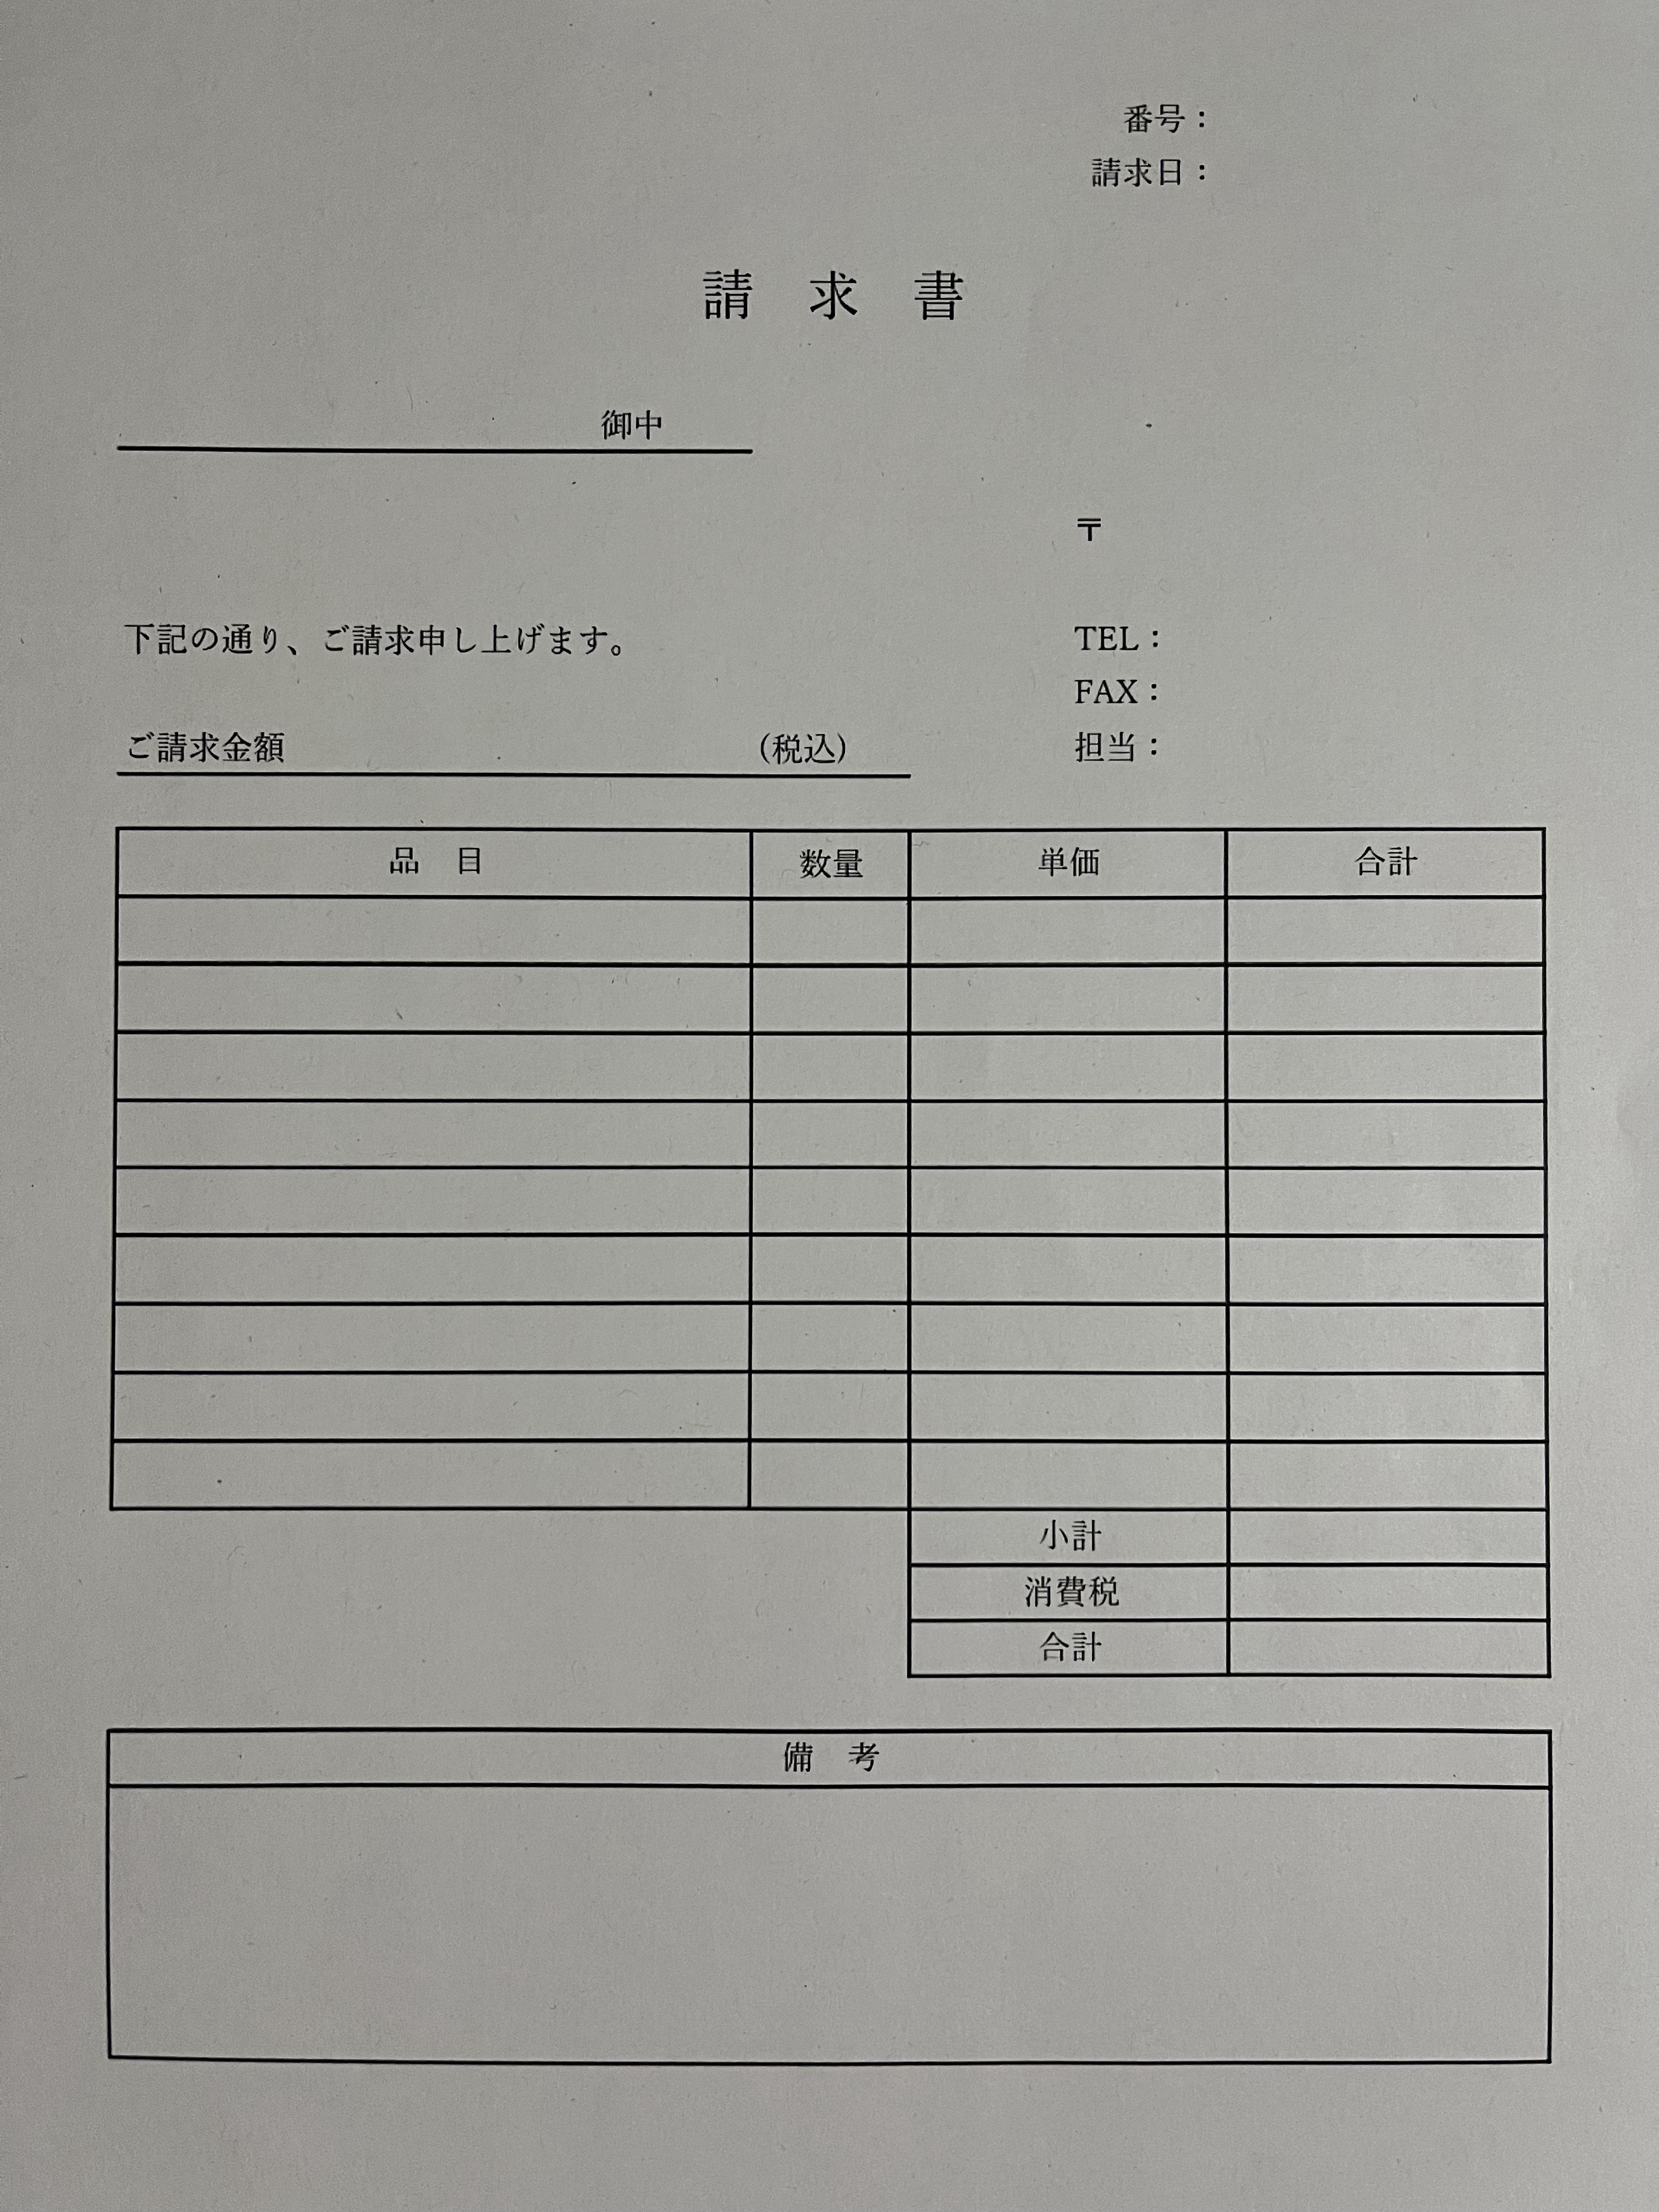
\includegraphics[width=15cm]{image/06-discussion/experiment_B.jpg}
        }
        \caption{実験対象である帳票画像B}
        \label{fig:experiment_B}
    \end{center}
\end{figure}

実験は、宮崎大学工学部情報システム工学科に所属する学部4年生X名、および修士1年生Y名、2年生Z名の計A名を対象として行った。

実験方法は、被験者A名を2つのグループに分け、片方のグループにケースAの実験を行い、もう片方のグループにケースBの実験を行う。
ケースAでは、図\ref{fig:experiment_A}の帳票画像に対して、本提案手法を適用せず、手作業で電子フォーム記入欄を配置してもらう。
次に、図\ref{fig:experiment_B}の帳票画像に対して、本提案手法を適用し、修正対象の電子フォーム記入欄を修正し、電子フォーム記入欄を配置してもらう。
ケースBでは、図\ref{fig:experiment_A}の帳票画像に対して、本提案手法を適用し、修正対象の電子フォーム記入欄を修正し、電子フォーム記入欄を配置してもらう。
次に、図\ref{fig:experiment_B}の帳票画像に対して、本提案手法を適用せず、手作業で電子フォーム記入欄を配置してもらう。

被験者が行った実験のケースを、以下の表に示す。

\begin{table}[tp]
	\centering
	\caption{被験者が行った実験ケースと手法}
    \label{tb:result}
    \begin{tabular}{cc}
        \begin{minipage}[c]{0.5\hsize}
            \centering
            \begin{tabular}{c|c}
                ケース & 被験者 \\
                \hline \hline
                \multirow{4}{*}{ケースA} & 被験者A \\
                                        & 被験者B \\
                                        & 被験者C \\
                                        & 被験者D \\
                                        \hline
                \multirow{4}{*}{ケースB} & 被験者E \\
                                        & 被験者F \\
                                        & 被験者G \\
                                        & 被験者H
	        \end{tabular}
        \end{minipage} &
        \begin{minipage}[c]{0.5\hsize}
            \centering
            \begin{tabular}{c|c|c}
                ケース & 帳票画像 & 手法 \\
                \hline \hline
                \multirow{2}{*}{ケースA} & 帳票画像A & 手作業のみ \\
                                        & 帳票画像B & 提案手法 + 修正 \\
                                        \hline
                \multirow{2}{*}{ケースB} & 帳票画像A & 提案手法 + 修正 \\
                                        & 帳票画像B & 手作業のみ
            \end{tabular}
        \end{minipage}
    \end{tabular}
\end{table}

なお、本提案手法で取得した領域座標、および、ラベルについては、間違っている可能性がある。
修正対象の電子フォーム記入欄に該当する電子フォーム記入欄を、以下に示す。

\begin{itemize}
    \item 誤検出によって、帳票画像内に帳票記入欄が存在しない場所に配置したもの。
    \item 帳票画像内に存在する帳票記入欄を検出できず、配置できていないもの。
    \item 本来想定するラベルとは異なるラベルを割り付けたもの。
\end{itemize}

実験で計測する時間について、本提案手法を適用し、JSONファイルと2枚の領域強調画像を出力するまでの時間を、実行時間と呼ぶ。
また、電子フォーム記入欄の配置が完了するまでの時間を、配置完了時間と呼ぶ。

実験の手順を、以下に示す。
なお、配置が必要な電子フォーム記入欄の数は、図\ref{fig:experiment_A}が65個、図\ref{fig:experiment_B}が48個である。

\begin{enumerate}
    \item 開始前に、実験対象の帳票画像とPhotolizeについて説明し、Photolizeにおける電子フォーム記入欄の配置操作も併せて説明する。
    \item 本提案手法を適用する場合は、実行時間を計測する。
    \item 適したラベルを考慮しつつ、電子フォーム記入欄の配置と修正をしてもらい、配置完了時間を計測する。
    \item 全電子フォーム記入欄の位置とラベルを確認し、正しく配置した割合を計算する。
\end{enumerate}

\subsection{電子フォーム記入欄の配置完了までにかかる時間に関する評価}\label{subsec:evalue_required_time}

\begin{table}[tp]
	\caption{}
	\label{tb:result}
	\centering
	\begin{tabular}{ccc||rrrr|r}
		被験者 & ケース & 帳票画像 & 実行時間 & 配置完了時間 & 合計 \\
        \hline \hline

		% 
		\multirow{2}{*}{被験者A} & \multirow{2}{*}{ケースA} & 帳票画像A &  & 00:19 & 00:34 \\
		                        &                          & 帳票画像B & 00:57 & 04:38 & 08:53 \\
                                                           \hline

		% 
		\multirow{2}{*}{被験者B} & \multirow{2}{*}{ケースA} & 帳票画像A &  & 00:19 & 00:34 \\
                                &                          & 帳票画像B & 00:57 & 04:38 & 08:53 \\
                                                           \hline

		%
		\multirow{2}{*}{被験者C} & \multirow{2}{*}{ケースA} & 帳票画像A &  & 00:19 & 00:34 \\
                                &                          & 帳票画像B & 00:57 & 04:38 & 08:53 \\
                                                           \hline

		%
		\multirow{2}{*}{被験者D} & \multirow{2}{*}{ケースA} & 帳票画像A &  & 00:19 & 00:34 \\
                                &                          & 帳票画像B & 00:57 & 04:38 & 08:53 \\
                                                           \hline

		%
		\multirow{2}{*}{被験者E} & \multirow{2}{*}{ケースB} & 帳票画像A & 00:57 & 00:19 & 00:34 \\
                                &                          & 帳票画像B & & 04:38 & 08:53 \\
                                                           \hline

		%
		\multirow{2}{*}{被験者F} & \multirow{2}{*}{ケースB} & 帳票画像A & 00:57 & 00:19 & 00:34 \\
                                &                         & 帳票画像B & & 04:38 & 08:53 \\
                                                           \hline
		%
		\multirow{2}{*}{被験者G} & \multirow{2}{*}{ケースB} & 帳票画像A & 00:57 & 00:19 & 00:34 \\
                                &                          & 帳票画像B & & 04:38 & 08:53 \\
                                                            \hline
		%
		\multirow{2}{*}{被験者H} & \multirow{2}{*}{ケースB} & 帳票画像A & 00:57 & 00:19 & 00:34 \\
                                &                          & 帳票画像B & & 04:38 & 08:53 \\
                                                            \hline
		\hline \hline
		% 平均
		\multirow{4}{*}{平均}  & \multirow{2}{*}{ケースA} & 帳票画像A &  & 00:19 & 00:34 \\
                               &                         & 帳票画像B & 00:57 & 04:38 & 08:53 \\
                               & \multirow{2}{*}{ケースB} & 帳票画像A &  & 00:19 & 00:34 \\
                               &                          & 帳票画像B & 00:57 & 04:38 & 08:53 \\
	\end{tabular}
\end{table}

\subsection{配置した電子フォーム記入欄の精度に関する評価}\label{subsec:evalue_accuracy}
本節では、配置した電子フォーム記入欄の精度について評価する。
なお、精度の評価は、領域座標の正解率、ラベルの正解率を算出することで行う。

領域座標の正解率と、ラベルの正解率を算出する式を、以下に示す。

\begin{equation}
    領域座標の正解率=\frac{正しく配置した電子フォーム記入欄の数}{帳票画像記入欄の数}
\end{equation}

\begin{equation}
    ラベルの正解率=\frac{正しくラベルを割り付けた電子フォーム記入欄の数}{帳票画像記入欄の数}
\end{equation}

理想は、手作業で配置した精度の100\%に近い精度が提案手法適用時にも出ること。



\section{関連研究}\label{sec:relation_research}



\section{本提案手法の問題点}\label{sec:AWSEL_problems}